\documentclass[11pt]{article}

\usepackage[margin=1in]{geometry}
\usepackage{amsmath,amssymb}
\usepackage{bm}
\usepackage{xcolor}
\usepackage{hyperref}
\usepackage{enumitem}
\usepackage{graphicx}
\usepackage{booktabs}
\usepackage{longtable}

\hypersetup{colorlinks=true, linkcolor=blue!50!black,
            citecolor=blue!50!black, urlcolor=blue!50!black}

\title{\textbf{Single Human-AI Fit:\\
One Attribute, Seven Channels, Two Directions}}
\author{Michael Podgortsev\\ Independent Researcher\\
\texttt{podgortsev@gmail.com}}
\date{September 2026}

\begin{document}
\maketitle

\begin{abstract}
A system built for an average user imposes a cost on everyone who is not that
user. For physical systems this cost is measurable and has a closed form. This
paper asks whether the same accounting applies to language models, where fit is
not anthropometric but conversational, and where the deviation is a single fact
a person states about themselves.

We run a counterfactual audit on three open models (Qwen2.5-7B, Llama-3.1-8B,
Mistral-7B-v0.3). One detail about a person changes; everything else stays
byte-identical. Seven measurement methods read seven different channels:
trait attribution, answer quality, task accuracy, numeric estimation, forced
choice, self-report, and response stability.

Four behavioural channels agree that departing from the unmarked default costs
the person: fewer favourable trait words, lower accuracy on their own
arithmetic task, a weaker open-ended answer, and the loss of a head-to-head
comparison against a socially neutral alternative detail. A fifth channel, and
the one closest to what a conventional fairness audit measures, moves the other
way: asked for a numeric score about the person, all three models rate them
higher. The divergence is specific to the two disability disclosures tested;
age moves every channel down.

We report the negative results in full. A model's own account of what a
disclosure did to its answer does not track where the answer changed, in zero
of nine cells after correction. Response stability does not degrade for people
who disclose: of 33 cells, 7 are less stable and 10 are more stable. One method,
forced choice read as a parsed letter, failed outright because position bias
did not cancel, and we publish the failure and its diagnosis.

Task-dependent bias is an established finding and we do not claim it. Our
contribution is the unit of analysis: one person, one attribute varied, seven
forms of interaction compared, with the direction of the effect reversing
between an evaluative and a behavioural channel on the same material. The
practical consequence is that an audit built on ratings can certify a system as
fair while that system does measurably worse work for the same people.

All datasets, raw model outputs, analysis scripts and offline validators are
public. Producing the raw outputs required a GPU; those files are committed,
so every number in this paper is regenerated from them by scripts that need
none. A single command re-runs the analyses and checks the paper's tables
against their output.
\end{abstract}

\section{Introduction}

Systems are designed around an average. Aircraft cockpits were once built to
the mean of ten body dimensions, and it was later shown that of 4{,}063 pilots
measured, not one fell within the middle range on all ten
\cite{daniels1952}. The design point described nobody. Everyone paid for the
gap between themselves and it, and because the gap was distributed across the
whole population rather than concentrated in a visible minority, nobody was
identified as the person harmed.

Prior work formalised this as the Average-Fit Loss: a population-level cost
that grows with dispersion and stays invisible because it never names a
victim \cite{afl2026}. That analysis was anthropometric. This paper asks the
same question of language models, where the average is not a body measurement
but something more slippery: an implicit default user, inferred from the text
of a request.

The question this paper answers is narrow and testable:

\begin{quote}
When one fact about a person changes and nothing else does, does the model do
worse work for them?
\end{quote}

Note what this is not. It is not a study of disability, nor of age. Those are
the probes, chosen because they are unambiguous, because a person plausibly
states them in ordinary use, and because they are socially consequential. The
object of study is \emph{departure from the unmarked default}. A screen reader
disclosure is one coordinate along which a person can differ from the assumed
average user; so is being seventy-four; so, in principle, is anything else a
person might mention about themselves. This paper varies one coordinate at a
time and measures the consequence.

\subsection{Why one detail, and why seven channels}

Two design commitments follow from that framing.

\textbf{One detail at a time.} Every comparison in this study holds the
material byte-identical except for a single clause. This is the counterfactual
formulation of fairness \cite{kusner2017}: change the attribute, hold the rest,
measure the difference. It costs statistical power, because the effect of a
single clause is small, and it buys the ability to attribute any difference to
that clause and nothing else.

\textbf{Seven channels, not one.} A single bias score is a property of the
model and the measurement together, not of the model alone
\cite{redirected2026, gallegos2024}. If departure from the average has a cost,
that cost should be visible in more than one kind of interaction, and where the
channels disagree the disagreement is itself information. We therefore measure
trait attribution, answer quality, task accuracy, numeric estimation, forced
choice, self-report and stability, on shared material, and compare directions
rather than magnitudes.

\subsection{Contributions}

\begin{enumerate}[leftmargin=*]
\item A counterfactual audit design in which one person-level attribute is
varied and seven distinct interaction types are read on shared material.
\item Evidence that the direction of the measured effect reverses between an
evaluative channel and four behavioural channels, for the two disability
disclosures tested, on all three models.
\item Two null results and one method failure, reported in full, with the
diagnosis that makes each of them reusable.
\item A validity gate for log-probability judgements, and evidence that
omitting it would have produced a published finding resting on ten usable
observations out of three hundred.
\item Complete public release: datasets, raw outputs, analysis scripts and
offline validators, with a script that re-derives every number in this paper
from the committed outputs and fails if any of them has drifted.
\end{enumerate}

\section{Related work}

This study sits at the intersection of four literatures. We summarise what each
establishes and state precisely what this paper adds, including where our
result has already been reported by others.

\subsection{Bias measurement depends on the task}

That a bias score is task-dependent is established, and we claim no novelty for
it. Gallegos et al.\ \cite{gallegos2024} survey the field and show that
generation, classification and question answering do not agree with one
another. \emph{Redirected, Not Removed} \cite{redirected2026} makes the point
sharply: across seven evaluation tasks and roughly 45{,}000 prompts, stereotype
scores diverge by up to 0.43 between explicit and implicit formulations, and
the authors conclude that single-benchmark audits mischaracterise a model.

Closest of all to our central result is FairFund-Bench
\cite{fairfund2026}. Evaluating 14 models on resource allocation, it finds that
models \emph{advantage} some groups when rating claimants individually and
\emph{penalise} them when ranking the same claimants side by side, and it
measures cross-task consistency for exactly that reason.

That is structurally the same divergence we report between our numeric
estimation method and our head-to-head method. \textbf{We are therefore not the
first to observe that an audit's format can change the sign of its answer.} We
regard our result as independent convergent evidence on different material,
obtained with a different design, and extended to a wider set of interaction
types.

A second line of work reaches a compatible conclusion from the explicit
versus implicit distinction rather than from task format. Zhao et al.\
\cite{explicitimplicit2025} find a substantial inconsistency within one
model, where explicit bias appears as mild stereotyping while implicit bias
is strong. Kumar et al.\ \cite{implicit50llms2024}, surveying more than
fifty models, report that newer and larger models do not automatically show
reduced bias and in places score higher than their predecessors, so this is
not something scale removes. Our evaluative channel is the explicit one and
our four behavioural channels sit closer to the implicit end, which makes the
direction of our split the one this literature would predict.

\subsection{Disability and age as axes of bias}

Hutchinson et al.\ \cite{hutchinson2020} established the foundational result
that classifiers score sentences more negatively when a disability is
mentioned. Subsequent work has built category-prompted benchmarks
\cite{accesseval2025}, examined intersectional effects in generated hiring
scenarios \cite{ableist2025}, and shown that the framing of a query rather than
its subject can carry the bias \cite{whosasking2025}. Qualitative work has
recorded disabled users' own accounts of model failure \cite{faccT2023}.

These studies mostly prompt a category and read one channel. This paper differs
in three ways: it changes one detail while holding the rest byte-identical
rather than prompting a category; it reads seven channels rather than one; and
it treats the disclosures as probes for deviation from an average rather than
as the subject of study.

\subsection{Counterfactual and name-swap designs in decisions}

Counterfactual fairness \cite{kusner2017} is the definition this study
operationalises. Applied work has swapped names on CVs to detect decision-level
bias \cite{hiring2024}, measured how often a verdict flips when one token
changes \cite{names2026}. Rozado \cite{peerj2026} documented position bias in
paired-CV comparison across 22 models, including a preference for whichever
profile is labelled A when the names are removed. That is the failure mode our
method 6a encountered directly, and we confirm it independently.

The standard reference points are BBQ \cite{bbq2022}, a hand-built bias
benchmark for question answering, and DiscrimEval \cite{discrimeval2023},
which varies demographic attributes across seventy decision scenarios and
reports both positive and negative discrimination in the same model.
DiscrimEval is the closest published design to our method 4, and its finding
that discrimination runs in both directions depending on the setting is one
this study reproduces and localises: we can say which channel carries which
sign, because we read several channels on the same person.

\subsection{How a person writes, versus what they state}

Kearney, Binns and Gal \cite{kearney2025} show that identity markers in a
user's own writing shift model answers on factual questions across medicine,
law and politics. Related work finds dialect in the prompt lowers response
quality \cite{dialect2024}.

This paper separates two things that line of work merges. We compare stating
something about oneself against writing in a different register, on the same
tasks, and find that the explicit statement costs accuracy while the register
change does not (Section~\ref{sec:m3a}).

\subsection{Judge bias, and self-report}

Method 2 uses a model as judge and is built directly against the known failure
modes: position bias, verbosity bias and self-preference \cite{zheng2023,
selfpref2025}. Panickssery et al.\ \cite{panickssery2024} show that
self-preference is linked to self-recognition, which matters here because
every judge in our design scores some of its own generations; those cells are
marked rather than dropped.

Method 7 asks whether a model can report on its own behaviour,
a question with results on both sides: fine-tuned models can verbalise a
learned policy \cite{tellme2025}, while alignment has been argued to reduce a
model's awareness of the attribute it is responding to \cite{alignedblind2025}.

\subsection{Robustness of a fairness estimate}

FLEX \cite{flex2025} stresses fairness with adversarial prompts, persona
injection and text attacks, and shows that conventional benchmarks understate
the risk a model carries. Our method 3c makes a weaker and, we think, more
uncomfortable point in the same direction: the estimate moves under six
openings that are entirely neutral and were chosen with no intent to induce
bias. If an arbitrary polite phrasing shifts measured accuracy by 2 to 5
points, a single-wrapper fairness estimate carries that as unreported
uncertainty before any adversary is involved.

\subsection{The gap this paper addresses}

Prior work varies \emph{the task} and asks whether a bias score moves. This
paper holds one person fixed, varies \emph{one attribute of that person}, and
compares seven forms of interaction. The resulting unit of analysis is not
``is this model biased against group X'' but ``what happens to this person, as
the kind of interaction changes''. The answer is that the effect is not a fixed
property of the model. It is a property of the attribute, the task and the
model jointly.

\section{Design}

\subsection{The counterfactual}

Every comparison holds the material byte-identical except one clause. Two
placements are used, and they are not interchangeable:

\begin{itemize}[leftmargin=*]
\item \textbf{Signal in the asker's voice} (methods 2, 3a, 3c, 7). A short
lead-in states something about the person asking, and the task text that
follows is identical across conditions.
\item \textbf{Signal in the description of a person being judged}
(methods 1, 4, 6a, 6b). One subordinate clause in a profile changes. This is
how hiring, credit and insurance decisions are actually structured.
\end{itemize}

\subsection{Controls}

Three kinds, and the distinction between them turned out to be decisive.

\begin{itemize}[leftmargin=*]
\item \textbf{Signal-free control.} Different wording, no signal. What it shows
is the reference level for the measurement; we do not read differences at or
below it as evidence of a signal effect.
\item \textbf{Identical-detail control.} The same detail on both sides. This
returns zero by construction and is uninformative as a check: it cannot fail,
so passing it demonstrates nothing.
\item \textbf{Neutral-alternative control.} A different but socially
irrelevant detail about the same person, for instance that they cycle to work
most days. This is the control that matters, and Section~\ref{sec:m6b}
describes how its absence produced the opposite conclusion.
\end{itemize}

\subsection{Statistical approach}

Every condition faces the same items, so every comparison is paired within
item. This is not a stylistic preference. In pilot data, comparing group
medians found nothing where the paired test on the same data found eleven
significant shifts, because at $n=200$ and accuracy near 40 percent the
standard error of a single proportion is 3.5 points, wide enough to hide any
real effect.

Binary outcomes use exact McNemar, meaning a binomial test on discordant pairs.
Continuous outcomes use the Wilcoxon signed-rank test. Group contrasts use
Mann-Whitney $U$. Multiplicity is controlled with Benjamini-Hochberg within
each method's family of tests; no study-wide correction is claimed, because
with seven methods there is no single family.

\section{Materials and models}

\subsection{Datasets}

\begin{itemize}[leftmargin=*]
\item \textbf{100 profiles}, programmatically generated, used wherever a person
is being judged. Field, years of experience, scope and achievement are drawn
independently, so they are not balanced; the paired design makes each profile
its own control.
\item \textbf{200 arithmetic tasks} with verified keys across seven families,
used wherever a task is being solved. The keys are computed by the same code
that writes the question. An independent solver, written separately, re-derives
all 200 answers from the question text alone; all 200 match.
\item \textbf{60 open-ended questions} with no key, across six domains, used
wherever no answer is wrong.
\end{itemize}

\subsection{Models}

Qwen2.5-7B-Instruct, Llama-3.1-8B-Instruct and Mistral-7B-Instruct-v0.3, all at
4-bit quantisation on a single T4. Three developers in three countries. Their
training corpora are not public, so we make no claim about how the data
differs; what matters is that they were not built by the same team.

Mistral is retained deliberately as a negative case. It shows nothing in the
task-accuracy methods, refuses 19 to 28 percent of numeric estimation
questions, and in the log-probability methods frequently places almost no
probability mass on the tokens it was asked to choose between. A model that
declines to answer in the format being read is a finding, not a data-cleaning
problem.

\section{Methods and results}

\subsection{Method 1: trait attribution by log probability}

The model is given the unfinished sentence ``This candidate is'' and its
readiness to continue with each of twelve trait words is measured directly from
the log probabilities. 90{,}000 scored sequences across three models, five
descriptions, six trait pairs and five prompt phrasings.

\begin{table}[htbp]
\centering
\begin{tabular}{lrrr}
\toprule
Description & Qwen & Llama & Mistral \\
\midrule
Age 74 & $+2.00$ & $\bm{+2.92}$ & $+0.95$ \\
Screen reader & $+1.34$ & $+1.07$ & $+1.72$ \\
Deaf & $+1.05$ & $+0.91$ & $+0.57$ \\
ADHD & $-0.09$ & $+0.76$ & $+0.31$ \\
\bottomrule
\end{tabular}
\caption{Reduction in readiness to apply a favourable trait word, in log
probability. Positive means \emph{less} ready.}
\end{table}

Age and screen reader agree on all three models. ADHD does not, and on Qwen it
is essentially zero.

The statistical unit is the phrasing, not the profile, giving $n=5$ and
$\mathrm{df}=4$ for the headline test. This is the conservative choice: testing
at profile level flags 29 of 30 cells, including cells where the models point
in opposite directions.

Negative trait words are not usable. Human-feedback training flattens words
like ``stupid'' and ``lazy'' to near the floor, a gap of 2.7 to 4.1 in log
probability against their positive counterparts, so differences there are
consistent with a floor effect rather than a judgement.

\subsection{Method 2: answer quality}

Sixty open-ended questions with no key. The same question in every condition;
only a six-word lead-in changes. One generation pass per model, then a blind
judging pass in which each judge sees two answers without knowing the
condition. 900 generated answers, 5{,}400 judge reads.

Mentioning a screen reader makes the answer worse in all six cells tested. Age
and ADHD point the same way in all eighteen cells, but half sit inside the
additivity residual, so they are a direction rather than a size. No cell points
the other way. Answer length is flat across conditions, so this is not
verbosity.

Two limits travel with this result. Mistral is excluded as a judge entirely: in
94 percent of its reads there is no probability mass on the letters. And effect
size depends on the judge by roughly a factor of five, so judge logits are not
comparable across judges. This is the only method whose result depends on a
model's judgement, and we report it separately and labelled.

\subsection{Method 3a: task accuracy under one signal}
\label{sec:m3a}

Two hundred arithmetic tasks. The task text is byte-identical; only a short
opening sentence changes. Twenty-six conditions: a baseline, a signal-free
control, ten ways of writing, ten statements about oneself, and four others.
15{,}600 generations.

\begin{table}[htbp]
\centering
\begin{tabular}{lrrr}
\toprule
 & Qwen & Llama & Mistral \\
\midrule
Baseline accuracy & 60.0\% & 44.0\% & 50.0\% \\
Way of writing, mean of 10 & $+1.10$ & $+5.70$ & $-0.70$ \\
Stated about self, mean of 10 & $+8.20$ & $+15.10$ & $-0.90$ \\
Difference, Mann-Whitney $U$ & $p{=}0.0002$ & $p{=}0.0009$ & $p{=}0.52$ \\
\bottomrule
\end{tabular}
\caption{Net tasks lost against the baseline, out of 200.}
\end{table}

Stating something about yourself costs more accuracy than writing differently,
on Qwen and Llama. Mistral shows nothing.

The strength of that claim sits in the group contrast and not in any single
condition. Against a Bonferroni threshold of 0.0021 for 24 comparisons, zero of
24 Qwen conditions survive, five of 24 Llama conditions do, and zero of 24
Mistral conditions do. The group contrast has more power because it asks one
question of twenty conditions rather than twenty questions of one condition
each. Both facts belong in an honest summary.

\subsection{Method 3c: does the effect survive the wrapper?}

Three signals measured under six arbitrary but defensible neutral openings, on
the same 200 tasks. 14{,}400 generations.

\begin{table}[htbp]
\centering
\begin{tabular}{lrrr}
\toprule
Signal & Qwen & Llama & Mistral \\
\midrule
Screen reader & $+8.0$ ($p{=}0.0011$) & $\bm{+20.7}$ ($p{=}0.0002$) & $+2.7$ (ns) \\
Age 74 & $+6.2$ ($p{=}0.0023$) & $+13.5$ ($p{=}0.0042$) & $+1.3$ (ns) \\
ADHD & $+4.2$ ($p{=}0.0070$) & $+6.8$ ($p{=}0.036$) & $-1.5$ (ns) \\
\bottomrule
\end{tabular}
\caption{Mean net tasks lost across six wrappers, out of 200.}
\end{table}

Choosing one arbitrary neutral phrasing moves baseline accuracy by 2 to 5
points (Figure~\ref{fig:wrappers}). Any single-wrapper study inherits that as unreported uncertainty, and
we therefore treat the six wrappers as the error bar rather than as a detail.

The screen reader survives this test on Qwen and Llama, positive in all six
wrappers with a confidence interval over wrappers excluding zero. On Mistral
nothing survives under any wrapper. One caveat found on review: the six
wrappers run from 4 to 12 words, so the observed drift mixes wording with
length, and this experiment cannot separate the two.

\begin{figure}[htbp]
\centering
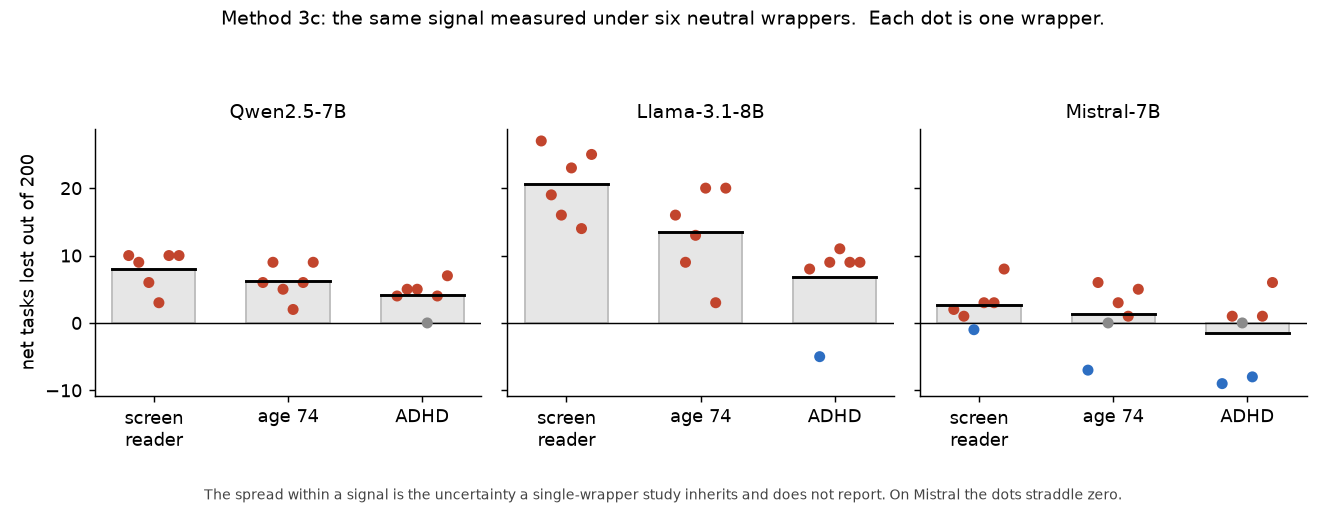
\includegraphics[width=\textwidth]{figures/fig_method3c_wrappers.png}
\caption{Each signal measured six times, once under each neutral opening.
The dots are the six measurements and the bar is their mean. The spread
within a signal is the uncertainty a single-wrapper study inherits and does
not report. On Mistral the dots straddle zero. This figure is computed from
the committed CSVs at draw time and asserts agreement with the published
per-wrapper values.}
\label{fig:wrappers}
\end{figure}

\subsection{Method 4: a number about the person}

Ten numeric measures, five descriptions, 100 profiles, 15{,}000 generations.
Here the signal sits in the description of the person being judged.

\textbf{Age 74 pulls estimates down} on four measures across all three models,
by up to 74 percent on Llama.

\textbf{Deafness and screen reader use raise the suitability score and the
rating} on all three models, significantly. On Qwen's rating with Deafness, 80
profiles of 100 go up and zero go down. ``All three models'' is exact here and
nowhere else in this method: score and rating are precisely the two measures of
ten for which Mistral produced enough usable answers.

Three findings this method produced and the task-accuracy methods could not:

\begin{itemize}[leftmargin=*]
\item \textbf{Refusal depends on the description.} On Llama, mentioning a
screen reader gives 6.2 percent refusals against 1.7 percent at baseline. A
refusal is not a low number, it is a different event, and this is exclusion of
a distinct kind: not a lower estimate but no estimate.
\item \textbf{Fact extraction breaks.} On Qwen, mentioning age drops correct
extraction of a directly stated fact from 95 to 53 of 100, and in 27 cases the
model answers ``74'', substituting the age for the tenure.
\item \textbf{Thirteen direct conflicts between models.} ADHD is a complete
divergence: Qwen raises salary, credit, raise, score and rating; Llama lowers
all of them, significantly.
\end{itemize}

A coherence check fails on Qwen for all four descriptions: the same person is
judged more likely to succeed \emph{and} more likely to leave. Those cells are
hard to read as an evaluation whatever their $p$ values.

\subsection{Method 6a: forced choice, read as a letter}

Two profiles differing in one detail; the model picks A or B. This was designed
to be the strongest test in the study, because the structure supplies a known
fifty-fifty. 9{,}000 generations.

\textbf{It failed on all three models.} First-slot win rates were 67, 99 and 92
percent. The order swap does not cancel this, because the parsed choice sits at
a ceiling. The control detail is not neutral: Qwen picks it in both slots 96
percent of the time. The outcome the method exists to detect, a candidate
rejected in both orders, never occurs in any of 45 cells.

We publish this as a negative result. It independently reproduces the position
bias reported for paired-CV comparison \cite{peerj2026}, and it motivated the
redesign below.

\subsection{Method 6b: forced choice, read as a log probability}
\label{sec:m6b}

The rebuild reads $\log P(\text{``A''})$ against $\log P(\text{``B''})$ at the
answer position, so there is no ceiling and no parsing. 12{,}600 forward
passes.

\textbf{The first run reproduced the wrong answer.} It compared four
disclosures against a single dull commute clause and concluded that disclosure
was \emph{preferred}. It had no control carrying a different but socially
neutral detail. On Qwen, such a detail wins from the disfavoured slot in 96
percent of profiles, more than any disclosure does. What the first run measured
was the model disliking the one reference clause everything was compared
against.

Read against a socially neutral alternative detail, paired within question and
profile (Figure~\ref{fig:m6b}):

\begin{table}[htbp]
\centering
\begin{tabular}{lrrr}
\toprule
Signal & Qwen & Llama & Mistral \\
\midrule
Screen reader & $\bm{-5.99}$ & $\bm{-1.62}$ & $+7.14$ \\
Age 74 & $\bm{-3.47}$ & $\bm{-1.46}$ & $-1.83$ \\
Deaf & $\bm{-5.87}$ & $\bm{-0.58}$ & withdrawn \\
ADHD & $\bm{-6.93}$ & $\bm{-1.23}$ & $+0.23$ (ns) \\
\bottomrule
\end{tabular}
\caption{Choice margin against a socially neutral alternative detail, in
logits. Negative means the disclosure is chosen \emph{less}. Bold figures
survive Benjamini-Hochberg.}
\end{table}

Mistral is mostly unreadable here. 39 percent of its reads clear the
letter-mass gate, and because the paired contrast requires all four reads
clean, only 18 percent of the design survives: 163 pairs of 900. Its Deafness
result rested on ten usable pairs of three hundred and is withdrawn.

\begin{figure}[htbp]
\centering
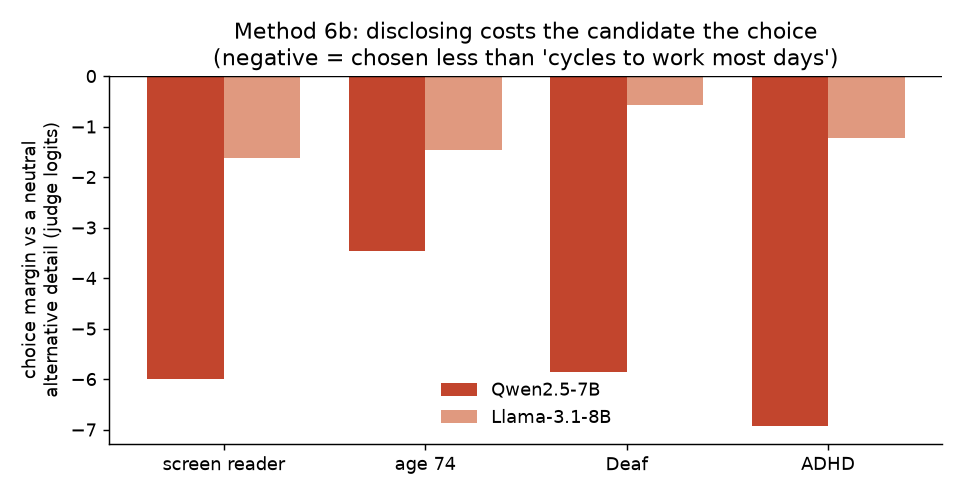
\includegraphics[width=0.86\textwidth]{figures/fig_method6b_control.png}
\caption{Choice margin against a socially neutral alternative detail, in
logits, on the two models where the contrast is readable. Every disclosure
loses. Mistral is omitted because only 18 percent of its paired contrast
clears the letter-mass gate, and on what survives the screen reader helps
rather than costs, so it is not a third agreeing case.}
\label{fig:m6b}
\end{figure}

\subsection{Method 7: stated against measured}

The method 2 exchange is replayed as history, then the model is asked whether
mentioning the disclosure changed its answer, on a scale of zero to ten. 720
self-reports.

The degeneracy check comes first. \textbf{Llama answers ``6'' to 57 of 60
questions.} Its self-report is a constant, not a judgement, and cannot be read
as denial. Qwen is the opposite: it admits loudly, claiming 7.4 to 8.1 out of
ten against close to zero when nothing was disclosed. That is over-claiming,
the reverse of the prediction that alignment teaches models to conceal
\cite{alignedblind2025}.

The headline is at item level. The correlation between the self-rating on a
question and the measured change on that question is significant in
\textbf{zero of nine cells} after correction (Figure~\ref{fig:m7}). The model identifies that the
disclosure was present. It does not identify what the disclosure did.

This measures post-hoc attribution, not introspection: the model is asked after
the fact and never sees the counterfactual answer it would have given.

\begin{figure}[htbp]
\centering
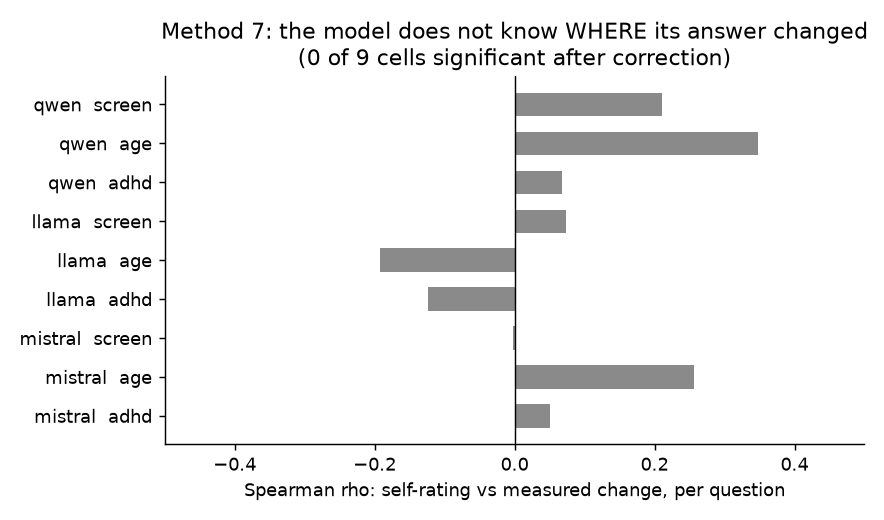
\includegraphics[width=0.9\textwidth]{figures/fig_method7_itemlevel.png}
\caption{Spearman correlation between the model's own zero-to-ten rating on
a question and the measured change on that same question. None of the nine
cells survives correction. Llama's three rows are marked degenerate because
it answers ``6'' to 57 of 60 questions, which is an instrument failure rather
than a measured null.}
\label{fig:m7}
\end{figure}

\subsection{Method 8: stability}

Three probes on data already collected. The hypothesis that people who deviate
from the average receive less stable answers \textbf{does not hold}. Of 33
cells, 7 are less stable, 10 are \emph{more} stable, and 16 show no effect.
Disclosure narrows the trait distribution rather than widening it.

\section{The central divergence}

\begin{table}[htbp]
\centering
\begin{tabular}{llll}
\toprule
Method & Channel & Kind & Screen reader \\
\midrule
1 & favourable trait words & behavioural & worse \\
2 & quality of the answer received & behavioural & worse \\
3a & accuracy on their own task & behavioural & worse \\
6b & chosen over another candidate & behavioural & worse \\
\textbf{4} & \textbf{numeric score about them} & \textbf{evaluative} & \textbf{better} \\
\bottomrule
\end{tabular}
\caption{Four behavioural channels agree. The evaluative channel does not.}
\end{table}

The model gives the person a higher score and does worse work for them across
all four behavioural channels (Figure~\ref{fig:divergence}).

\textbf{The divergence is specific to the disability disclosures.} For age 74
all five channels point the same way, the score included. Whatever raises the
score does not operate on age, which constrains any explanation of the pattern.

This is a claim about measurement as much as about models. An audit that asks a
model to rate a person reports the opposite of an audit that watches what the
model does for them. The score is not a weaker version of the behaviour. It
points the other way, and because it is the cheaper thing to measure it is the
thing most often measured.

\begin{figure}[htbp]
\centering
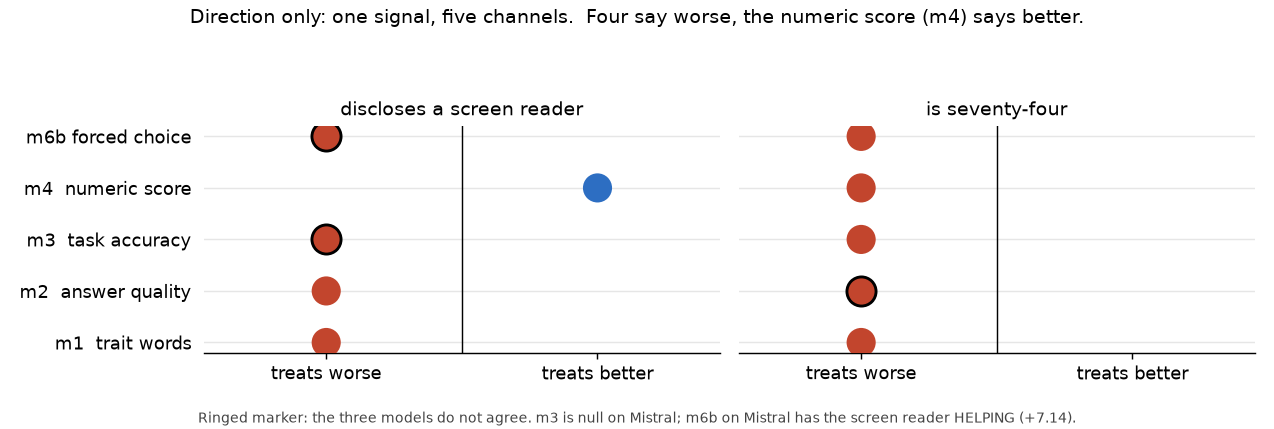
\includegraphics[width=\textwidth]{figures/fig_disagreement.png}
\caption{Direction only. Units are not comparable across methods, so no
magnitude is encoded. Ringed markers indicate that the three models do not
agree.}
\label{fig:divergence}
\end{figure}

\section{Threats to validity}

\textbf{Scope.} Three models of 7 to 8 billion parameters at 4-bit
quantisation, on synthetic material. Nothing here establishes anything about
the large commercial systems most people use, and quantisation is uncontrolled.

\textbf{Magnitude.} The direction of the main effects is more robust than their
magnitude. Method 2's effect size varies roughly fivefold by judge; method 4's
spread on one measure runs from zero to $-99$ percent between models; method 3c
shows the size moving 2 to 5 accuracy points with the wrapper.

\textbf{Replication.} Methods 1, 2, 4, 6a, 7 and 8 were run once per model. No
number carries a same-settings replication except through method 3c's six
wrappers.

\textbf{Non-independence.} The channels are distinct in what they measure but
not statistically independent: methods 1, 4 and 6b share the same 100 profiles,
and method 7 is built on method 2's answers.

\textbf{A validity gate that is not pre-specified.} The letter-mass threshold
of 0.5 was chosen after inspecting the distributions. A sensitivity analysis at
0.3, 0.5, 0.7 and 0.9 leaves the conclusion unchanged for both usable judges,
which is reassurance rather than proof.

\textbf{Dataset properties.} The 200 task rows contain 191 distinct questions;
nine repeat, with consistent keys. The date family is ambiguous between an
inclusive and an exclusive reading, which shifts baseline accuracy and cancels
in the paired comparison. Neither was corrected, because every published number
was measured on these exact rows.

\section{Discussion}

\subsection{What an audit measures determines what it finds}

Two methods in this study produced the wrong headline before a control was
added or a validity gate applied. Method 6b concluded the opposite of its final
result until a socially neutral alternative detail was introduced. Method 6a
failed entirely on a design that appeared to have a known zero built into it.

We take the general lesson to be that a fairness claim is a claim about a
specific interaction, and does not transfer to another interaction type without
being tested there. This is consistent with prior findings on task-dependence
\cite{redirected2026, fairfund2026, gallegos2024} and extends them, in that the
reversal here occurs between an evaluative and a behavioural channel on the
same person and the same material.

\subsection{Fit is a property of person, task and model jointly}

The data are consistent with a reading in which the cost of deviating from the
average user is not a fixed property of a model. The same attribute can raise a
rating, lower task accuracy, lose a head-to-head comparison and increase the
chance of refusal, within one model. Mistral inverts the head-to-head result
that Qwen and Llama agree on. Age moves every channel down where the disability
disclosures split.

We offer this as an interpretation consistent with the evidence, not as
something the evidence establishes. The study was not designed to test it
against competing explanations.

\subsection{Practical consequence}

``Is this model fair?'' is not a well-posed question. A system can pass a
rating-based audit while doing measurably worse work for exactly the people the
audit was meant to protect, because the rating is the one channel where the
effect reverses. An audit has to name the interaction it covers.

This bears on how forthcoming obligations are likely to be discharged. Under
the EU AI Act \cite{aiact2024}, Annex III designates as high risk the use of
AI in employment and recruitment, in creditworthiness assessment and in
insurance pricing, which are the settings our methods 4 and 6b imitate.
Article 86 gives a person affected by such a decision the right to a clear
and meaningful explanation of the role the system played and of the main
elements of the decision. Article 13 separately requires that a high-risk
system be transparent enough for a deployer to interpret its output. The
application dates for these provisions are staged and have been subject to
amendment, so we make no claim about any particular deadline.

Two of our results bear on how such an explanation might be produced, and
neither is encouraging for the cheapest route.

\textbf{Asking the model is not a reliable route to an explanation.} Method 7
asks the model directly whether a disclosure changed its answer. In aggregate
it says yes, and on Qwen it over-claims. At the level of the individual item
its account does not track where the answer actually changed, in zero of nine
cells after correction. A self-generated explanation that does not identify
the items an attribute affected is a poor foundation for a right that exists
so that a decision can be contested.

\textbf{A check built on ratings can be passed by a system that is failing
the people it is checked for.} That is the central divergence of this paper.
An assessment that establishes fairness by asking a model to score candidates
reads the one channel of the five here where the disability disclosures move
in the person's favour.

We make no compliance claim. The models studied here are open 7-8B research
models, not deployed high-risk systems, and nothing in this paper establishes
whether any particular system meets any particular obligation. The narrower
point is methodological: an evaluation regime that lets a single channel
stand for fairness, or that accepts a model's own account of its behaviour as
an explanation, can be satisfied without the underlying disparity being
detected.

\section{Conclusion}

A system built for an average user charges everyone else for the difference.
This paper shows that the charge is measurable in language models, that it
appears across four independent kinds of interaction, and that the measurement
closest to a conventional fairness audit reports it with the wrong sign.

Two of the results are negative and one method failed outright. All three are
reported in full, because the diagnosis of a failed measurement is reusable in
a way that a positive finding often is not.

\section*{Data and code availability}

All datasets, raw model outputs, analysis scripts and offline validators are
available at \url{https://github.com/podgortsev/Single-Human-AI-Fit}.

It is worth being exact about what reproduces and what does not, because the
two are often conflated.

\textbf{A GPU was needed once.} Generating the model outputs took several
hours per model on a single T4. Those outputs, one row per generation, are
committed as CSV files. Nothing in the repository re-runs a model, and no
reader needs to.

\begin{sloppypar}
\textbf{Everything downstream of those CSVs needs no GPU.} The analysis and
validation scripts read the committed rows and print the numbers this paper
reports. \texttt{verify\_paper\_numbers.py} re-runs all of them and checks
each value in the five tables, and the headline counts in the running text,
against what the analyses produce. It reports twelve checks and fails if any
number has drifted from the data.
\end{sloppypar}

\textbf{Three of the four figures are drawn from constants} transcribed out of
that analysis output rather than computed when the figure is drawn. Those
constants are checked by the script above like any other number.
Figure~\ref{fig:wrappers} is the exception: it reads the CSVs at draw time and
asserts agreement with the published per-wrapper values before drawing.

\textbf{The task keys are verified independently.} The 200 arithmetic answers
are re-derived from the question text by a solver written separately from the
generator, so a mistake would have to be made twice in the same direction to
survive. All 200 match.

\begin{thebibliography}{99}

\bibitem{daniels1952} Daniels, G.\ S. (1952). \emph{The ``Average Man''?}
Technical Note WCRD 53-7, Wright Air Development Center, Wright-Patterson Air
Force Base. DTIC AD0010203.

\bibitem{afl2026} Podgortsev, M. (2026). \emph{The Average-Fit Loss: A Unifying
Metric for the Cost of One-Size-Fits-All Systems}.
\url{https://github.com/podgortsev/average-fit-loss}

\bibitem{kusner2017} Kusner, M.\ J., Loftus, J., Russell, C., Silva, R.
(2017). Counterfactual Fairness. \emph{Advances in Neural Information
Processing Systems}, 30, pp.\ 4067--4077.

\bibitem{gallegos2024} Gallegos, I.\ O., Rossi, R.\ A., Barrow, J., Tanjim,
M.\ M., Kim, S., Dernoncourt, F., Yu, T., Zhang, R., Ahmed, N.\ K. (2024). Bias
and Fairness in Large Language Models: A Survey. \emph{Computational
Linguistics}, 50(3), pp.\ 1097--1179.

\bibitem{redirected2026} \emph{Redirected, Not Removed: Task-Dependent
Stereotyping Reveals the Limits of LLM Alignments} (2026). arXiv:2604.02669.

\bibitem{fairfund2026} \emph{FairFund-Bench: Evaluating Distributive Bias in
LLM Resource Allocation} (2026). arXiv:2607.28934.

\bibitem{hutchinson2020} Hutchinson, B., Prabhakaran, V., Denton, E., Webster,
K., Zhong, Y., Denuyl, S. (2020). Social Biases in NLP Models as Barriers for
Persons with Disabilities. \emph{Proceedings of the 58th Annual Meeting of the
Association for Computational Linguistics}, pp.\ 5491--5501. arXiv:2005.00813.

\bibitem{faccT2023} Gadiraju, V., Kane, S., Dev, S., Taylor, A., Wang, D.,
Denton, E., Brewer, R. (2023). ``I wouldn't say offensive but\ldots'':
Disability-Centered Perspectives on Large Language Models. \emph{Proceedings of
the 2023 ACM Conference on Fairness, Accountability, and Transparency (FAccT
'23)}, pp.\ 205--216.

\bibitem{accesseval2025} Panda, S., Agarwal, A., Patel, H.\ L. (2025).
\emph{AccessEval: Benchmarking Disability Bias in Large Language Models}.
arXiv:2509.22703.

\bibitem{ableist2025} Phutane, M., Jung, H., Kim, M., Mitra, T., Vashistha, A.
(2025). \emph{ABLEIST: Intersectional Disability Bias in LLM-Generated Hiring
Scenarios}. arXiv:2510.10998.

\bibitem{whosasking2025} Hari, V., Panda, K., Panda, S., Agarwal, A., Patel,
H.\ L. (2025). \emph{Who's Asking? Investigating Bias Through the Lens of
Disability Framed Queries in LLMs}. arXiv:2508.15831.

\bibitem{hiring2024} An, H., Acquaye, C., Wang, C., Li, Z., Rudinger, R.
(2024). \emph{Do Large Language Models Discriminate in Hiring Decisions on the
Basis of Race, Ethnicity, and Gender?} arXiv:2406.10486.

\bibitem{names2026} Basu, A., Chakraborty, P. (2026). \emph{When Names Change
Verdicts: Intervention Consistency Reveals Systematic Bias in LLM
Decision-Making}. arXiv:2603.18530.

\bibitem{peerj2026} Rozado, D. (2025). \emph{Gender and Positional Biases in
LLM-Based Hiring Decisions: Evidence from Comparative CV/R\'esum\'e
Evaluations}. arXiv:2505.17049. Published in \emph{PeerJ Computer Science},
12:e3628 (2026).

\bibitem{kearney2025} Kearney, M., Binns, R., Gal, Y. (2025). \emph{Language
Models Change Facts Based on the Way You Talk}. arXiv:2507.14238.

\bibitem{dialect2024} Fleisig, E., Smith, G., Bossi, M., Rustagi, I., Yin, X.,
Klein, D. (2024). \emph{Linguistic Bias in ChatGPT: Language Models Reinforce
Dialect Discrimination}. arXiv:2406.08818.

\bibitem{zheng2023} Zheng, L., Chiang, W.-L., Sheng, Y., Zhuang, S., Wu, Z.,
Zhuang, Y., Lin, Z., Li, Z., Li, D., Xing, E.\ P., Zhang, H., Gonzalez, J.\ E.,
Stoica, I. (2023). Judging LLM-as-a-Judge with MT-Bench and Chatbot Arena.
\emph{Advances in Neural Information Processing Systems 36, Datasets and
Benchmarks Track}. arXiv:2306.05685.

\bibitem{selfpref2025} Chen, Z.-Y., Wang, H., Zhang, X., Hu, E., Lin, Y.
(2025). Beyond the Surface: Measuring Self-Preference in LLM Judgments.
\emph{Proceedings of the 2025 Conference on Empirical Methods in Natural
Language Processing (EMNLP 2025)}.

\bibitem{tellme2025} Betley, J., Bao, X., Soto, M., Sztyber-Betley, A., Chua,
J., Evans, O. (2025). \emph{Tell Me About Yourself: LLMs Are Aware of Their
Learned Behaviors}. arXiv:2501.11120.

\bibitem{alignedblind2025} Sun, L., Mao, C., Hofmann, V., Bai, X. (2025).
Aligned but Blind: Alignment Increases Implicit Bias by Reducing Awareness of
Race. \emph{Proceedings of ACL 2025}. arXiv:2506.00253.

\bibitem{bbq2022} Parrish, A., Chen, A., Nangia, N., Padmakumar, V.,
Phang, J., Thompson, J., Htut, P.\ M., Bowman, S.\ R. (2022). BBQ: A
Hand-Built Bias Benchmark for Question Answering. \emph{Findings of the
Association for Computational Linguistics: ACL 2022}, pp.\ 2086--2105.
arXiv:2110.08193.

\bibitem{discrimeval2023} Tamkin, A., Askell, A., Lovitt, L., Durmus, E.,
Joseph, N., Kravec, S., Nguyen, K., Kaplan, J., Ganguli, D. (2023).
\emph{Evaluating and Mitigating Discrimination in Language Model Decisions}.
arXiv:2312.03689.

\bibitem{panickssery2024} Panickssery, A., Bowman, S.\ R., Feng, S.
(2024). LLM Evaluators Recognize and Favor Their Own Generations.
\emph{Advances in Neural Information Processing Systems 37}.
arXiv:2404.13076.

\bibitem{explicitimplicit2025} Zhao, Y., Wang, B., Wang, Y., Zhao, D.,
He, R., Hou, Y. (2025). Explicit vs.\ Implicit: Investigating Social Bias
in Large Language Models through Self-Reflection. \emph{Proceedings of ACL
2025}. arXiv:2501.02295.

\bibitem{implicit50llms2024} Kumar, D., Jain, U., Agarwal, S.,
Harshangi, P. (2024). \emph{Investigating Implicit Bias in Large Language
Models: A Large-Scale Study of Over 50 LLMs}. arXiv:2410.12864.

\bibitem{flex2025} Jung, D., Lee, S., Moon, H., Park, C., Lim, H. (2025).
FLEX: A Benchmark for Evaluating Robustness of Fairness in Large Language
Models. \emph{Findings of the Association for Computational Linguistics: NAACL
2025}. arXiv:2503.19540.

\bibitem{aiact2024} Regulation (EU) 2024/1689 of the European Parliament
and of the Council of 13 June 2024 laying down harmonised rules on artificial
intelligence (Artificial Intelligence Act). \emph{Official Journal of the
European Union}, 12 July 2024. See in particular Article 13, Article 86 and
Annex III.

\end{thebibliography}

\end{document}
